\documentclass[twocolumn]{article}
\usepackage{lmodern}
\usepackage{amssymb,amsmath}
\usepackage{ifxetex,ifluatex}
\usepackage{fixltx2e} % provides \textsubscript
\ifnum 0\ifxetex 1\fi\ifluatex 1\fi=0 % if pdftex
  \usepackage[T1]{fontenc}
  \usepackage[utf8]{inputenc}
\else % if luatex or xelatex
  \ifxetex
    \usepackage{mathspec}
    \usepackage{xltxtra,xunicode}
  \else
    \usepackage{fontspec}
  \fi
  \defaultfontfeatures{Mapping=tex-text,Scale=MatchLowercase}
  \newcommand{\euro}{€}
\fi
% use upquote if available, for straight quotes in verbatim environments
\IfFileExists{upquote.sty}{\usepackage{upquote}}{}
% use microtype if available
\IfFileExists{microtype.sty}{%
\usepackage{microtype}
\UseMicrotypeSet[protrusion]{basicmath} % disable protrusion for tt fonts
}{}
\usepackage[margin=2cm]{geometry}
\ifxetex
  \usepackage[setpagesize=false, % page size defined by xetex
              unicode=false, % unicode breaks when used with xetex
              xetex]{hyperref}
\else
  \usepackage[unicode=true]{hyperref}
\fi
\hypersetup{breaklinks=true,
            bookmarks=true,
            pdfauthor={Greg Gloor},
            pdftitle={Supplementary workflow},
            colorlinks=true,
            citecolor=blue,
            urlcolor=blue,
            linkcolor=magenta,
            pdfborder={0 0 0}}
\urlstyle{same}  % don't use monospace font for urls
\usepackage{color}
\usepackage{fancyvrb}
\newcommand{\VerbBar}{|}
\newcommand{\VERB}{\Verb[commandchars=\\\{\}]}
\DefineVerbatimEnvironment{Highlighting}{Verbatim}{commandchars=\\\{\}}
% Add ',fontsize=\small' for more characters per line
\usepackage{framed}
\definecolor{shadecolor}{RGB}{248,248,248}
\newenvironment{Shaded}{\begin{snugshade}}{\end{snugshade}}
\newcommand{\KeywordTok}[1]{\textcolor[rgb]{0.13,0.29,0.53}{\textbf{{#1}}}}
\newcommand{\DataTypeTok}[1]{\textcolor[rgb]{0.13,0.29,0.53}{{#1}}}
\newcommand{\DecValTok}[1]{\textcolor[rgb]{0.00,0.00,0.81}{{#1}}}
\newcommand{\BaseNTok}[1]{\textcolor[rgb]{0.00,0.00,0.81}{{#1}}}
\newcommand{\FloatTok}[1]{\textcolor[rgb]{0.00,0.00,0.81}{{#1}}}
\newcommand{\ConstantTok}[1]{\textcolor[rgb]{0.00,0.00,0.00}{{#1}}}
\newcommand{\CharTok}[1]{\textcolor[rgb]{0.31,0.60,0.02}{{#1}}}
\newcommand{\SpecialCharTok}[1]{\textcolor[rgb]{0.00,0.00,0.00}{{#1}}}
\newcommand{\StringTok}[1]{\textcolor[rgb]{0.31,0.60,0.02}{{#1}}}
\newcommand{\VerbatimStringTok}[1]{\textcolor[rgb]{0.31,0.60,0.02}{{#1}}}
\newcommand{\SpecialStringTok}[1]{\textcolor[rgb]{0.31,0.60,0.02}{{#1}}}
\newcommand{\ImportTok}[1]{{#1}}
\newcommand{\CommentTok}[1]{\textcolor[rgb]{0.56,0.35,0.01}{\textit{{#1}}}}
\newcommand{\DocumentationTok}[1]{\textcolor[rgb]{0.56,0.35,0.01}{\textbf{\textit{{#1}}}}}
\newcommand{\AnnotationTok}[1]{\textcolor[rgb]{0.56,0.35,0.01}{\textbf{\textit{{#1}}}}}
\newcommand{\CommentVarTok}[1]{\textcolor[rgb]{0.56,0.35,0.01}{\textbf{\textit{{#1}}}}}
\newcommand{\OtherTok}[1]{\textcolor[rgb]{0.56,0.35,0.01}{{#1}}}
\newcommand{\FunctionTok}[1]{\textcolor[rgb]{0.00,0.00,0.00}{{#1}}}
\newcommand{\VariableTok}[1]{\textcolor[rgb]{0.00,0.00,0.00}{{#1}}}
\newcommand{\ControlFlowTok}[1]{\textcolor[rgb]{0.13,0.29,0.53}{\textbf{{#1}}}}
\newcommand{\OperatorTok}[1]{\textcolor[rgb]{0.81,0.36,0.00}{\textbf{{#1}}}}
\newcommand{\BuiltInTok}[1]{{#1}}
\newcommand{\ExtensionTok}[1]{{#1}}
\newcommand{\PreprocessorTok}[1]{\textcolor[rgb]{0.56,0.35,0.01}{\textit{{#1}}}}
\newcommand{\AttributeTok}[1]{\textcolor[rgb]{0.77,0.63,0.00}{{#1}}}
\newcommand{\RegionMarkerTok}[1]{{#1}}
\newcommand{\InformationTok}[1]{\textcolor[rgb]{0.56,0.35,0.01}{\textbf{\textit{{#1}}}}}
\newcommand{\WarningTok}[1]{\textcolor[rgb]{0.56,0.35,0.01}{\textbf{\textit{{#1}}}}}
\newcommand{\AlertTok}[1]{\textcolor[rgb]{0.94,0.16,0.16}{{#1}}}
\newcommand{\ErrorTok}[1]{\textcolor[rgb]{0.64,0.00,0.00}{\textbf{{#1}}}}
\newcommand{\NormalTok}[1]{{#1}}
\usepackage{graphicx,grffile}
\makeatletter
\def\maxwidth{\ifdim\Gin@nat@width>\linewidth\linewidth\else\Gin@nat@width\fi}
\def\maxheight{\ifdim\Gin@nat@height>\textheight\textheight\else\Gin@nat@height\fi}
\makeatother
% Scale images if necessary, so that they will not overflow the page
% margins by default, and it is still possible to overwrite the defaults
% using explicit options in \includegraphics[width, height, ...]{}
\setkeys{Gin}{width=\maxwidth,height=\maxheight,keepaspectratio}
\setlength{\parindent}{0pt}
\setlength{\parskip}{6pt plus 2pt minus 1pt}
\setlength{\emergencystretch}{3em}  % prevent overfull lines
\providecommand{\tightlist}{%
  \setlength{\itemsep}{0pt}\setlength{\parskip}{0pt}}
\setcounter{secnumdepth}{0}

%%% Use protect on footnotes to avoid problems with footnotes in titles
\let\rmarkdownfootnote\footnote%
\def\footnote{\protect\rmarkdownfootnote}

%%% Change title format to be more compact
\usepackage{titling}

% Create subtitle command for use in maketitle
\newcommand{\subtitle}[1]{
  \posttitle{
    \begin{center}\large#1\end{center}
    }
}

\setlength{\droptitle}{-2em}
  \title{Supplementary workflow}
  \pretitle{\vspace{\droptitle}\centering\huge}
  \posttitle{\par}
  \author{Greg Gloor}
  \preauthor{\centering\large\emph}
  \postauthor{\par}
  \predate{\centering\large\emph}
  \postdate{\par}
  \date{17 January, 2018}

% Redefines (sub)paragraphs to behave more like sections
\ifx\paragraph\undefined\else
\let\oldparagraph\paragraph
\renewcommand{\paragraph}[1]{\oldparagraph{#1}\mbox{}}
\fi
\ifx\subparagraph\undefined\else
\let\oldsubparagraph\subparagraph
\renewcommand{\subparagraph}[1]{\oldsubparagraph{#1}\mbox{}}
\fi

\usepackage{amsmath}
\newcommand{\ith}[1]{ #1\textsuperscript{th}\ }
\newcommand{\vect}[1]{\vec{\textbf{#1}}}

\begin{document}
\maketitle

{
\hypersetup{linkcolor=black}
\setcounter{tocdepth}{2}
\tableofcontents
}
\section{About this document}\label{about-this-document}

This document is an .Rmd document and can be found at:

github.com/ggloor/templates

The document is a template for two column R markdown. It requires an
installation of \LaTeX to work properly. This document can contain
interspersed markdown and R code that may be compiled into a pdf
document and supports the figures and assertions in the main article. R
code is not exposed in the pdf document but is referred to by
\texttt{R\ code\ block} in the text so that the interested reader can
work through the example code themselves.

\subsection{Reproducing the analysis}\label{reproducing-the-analysis}

From an R command prompt you can compile this document into PDF if you
have \LaTeX and pandoc installed:

\texttt{rmarkdown::render(\textquotesingle{}two\_column.Rmd\textquotesingle{})}
or you can open the file in RStudio and compile in that environment.

\subsection{R packages required}\label{r-packages-required}

We will need the following R packages and add-ons
(\texttt{R\_block\_1}).

\begin{enumerate}
\def\labelenumi{\arabic{enumi}.}
\tightlist
\item
  knitr (CRAN)
\end{enumerate}

\clearpage

\section{Common data transforms in high throughput
sequencing}\label{common-data-transforms-in-high-throughput-sequencing}

Fundamentally, the goal of any experiment is to determine something
about the environment that was sampled. After all, we are attempting to
use HTS to determine something of interest about the underlying
environment. Thus, we need to have some equivalence between the samples
before sequencing and the samples after sequencing. The simplest case
would be that there would be a linear relationship between the data that
we could obtain from the environment, and the data that was actually
collected by HTS.

We can think about the underlying data on a univariate basis; do the
features across all samples follow a Gaussian distribution? or do they
follow some unknown distribution? If so, can we transform the data to
approximate a Gaussian distribution? This mode of thinking leads to the
use of square-root, arcsine or Hellinger transformations since they
appear to transform the data into a distribution that can be
interpreted. However, as we shall see below, none of these univariate
transformations is suitable.

It is more desirable to think about HTS data in a multivariate way as a
`composition' because the total count of molecules in the underlying
sample (the environment) is always a confounding variable (Lovén et al.,
2012). This way of thinking led to multivariate data normalizations.

\subsection{Notation}\label{notation}

We use the following notation throughout. Column vectors contain samples
\(\vec{\textbf{s}}\) and row vectors contain features
\(\vec{\textbf{f}}\). There are \(D\) features and \(n\) samples, thus
the data are contained in matrix \(M = D \times n\). The \(j^{th}\)
sample is denoted as \(s_{j}\), the \(i^{th}\) feature of all samples is
denoted as \(s_{i-}\), and the value for the \(i^{th}\) feature of the
\(j^{th}\) sample is referred to as \(s_{ij}\).

\subsection{Simple proportional type
transformations}\label{simple-proportional-type-transformations}

The simplest normalization is to determine the relative abundance (rAB),
or proportion, of the \ith{i} feature in a sample as in Eq.
\ref{eq:rab}.

\begin{equation}
    rAB_{i} = \frac{s_{i}}{\sum{\vec{\textbf{s}}}}
    \label{eq:rab}
\end{equation}

This normalization is also referred to as the total sum scaling (TSS)
normalization. The rAB measure requires only the read count observed for
a the feature \(s_i\) and the total read count of the sample
\(\sum{\vec{\textbf{s}}}\). Since this measure is generally skewed, it
is often log-transformed prior to analysis.

A further normalization was proposed early in the RNA-seq field where
the reads per kilobase per million mapped (RPKM)(Mortazavi et al., 2008)
method was used initially to place the read counts for each feature
within and between samples on a common scale.

For this we also needed to know a scaling factor \(K\), and the length
of the feature \(L_i\); from this, the RPKM value for the \ith{i}
feature for each sample was calculated as in Eq. \ref{eq:rpkm}.

\begin{equation}
    RPKM_{i} = \frac{(K \cdot C_{i} )}{\sum{C} \cdot L_{i}}
    \label{eq:rpkm}
\end{equation}

When the equation is placed in this form it is obvious that RPKM is
simply a scaled rAB where each rAB value is divided by its length
multiplied by a constant. In compositional terms, RPKM is an unclosed
perturbation of the original data.

Further research suggested that RPKM was not appropriate for comparison
of features between samples. The goal of RPKM was to `count' reads per
feature per cell. In the original paper the authors supplied an
equivalence and an RPKM value of 1 RPKM equalled one transcript in each
cell in the C2C12 cell line, but in liver cells, a value of 3 RPKM
equalled one transcript per cell. Thus, from the start, this
normalization was unable to normalize between-condition read counts.

The transcripts per million (TPM) normalization was advocated next (Li
et al., 2010). Patcher (Pachter, 2011) showed the equivalence between
RPKM and TPM, and in compositional terms TPM is simply a compositionally
closed form of RPKM multiple by a constant as in Eq. \ref{eq:tpm}.

\begin{equation}
    TPM_{i} = \frac{RPKM_i}{\sum{RPKM}} \cdot K
    \label{eq:tpm}
\end{equation}

The rAB, RPKM and TPM normalizations are thus all very similar,
differing only in the scaling of individual features, and do not allow
normalization between conditions unless the conditions contain the same
input number of RNA molecules. In a very real sense, these
normalizations deliver proportional data, scaled or perturbed to make
the data appear as if they are numerical, and not proportional.

A related transformation is `rarefaction' or subsampling without
replacement to a defined per-sample read count. This transformation was
widely used in the 16S rRNA gene sequencing field. Rarefaction to a
common read count gives a composition, that is scaled such that low
count features often are replaced by 0 values (McMurdie and Holmes,
2014). For this reason, rarefaction has now been largely replaced with
the median of ratios method described below.

\subsection{The median of ratios count
normalization}\label{the-median-of-ratios-count-normalization}

Further work found that none of these methods were appropriate, since
the read count per sample continued to confound the analyses (Lovén et
al., 2012). Thus, the scaling normalization methods were proposed
(Robinson and Oshlack, 2010). There are two main scaling normalizations,
but both operate on the common assumption that by normalizing all counts
in a sample to a midpoint of each sample that the normalization can
impute the \emph{number} of each feature in the environment. The
approaches differ largely in how the midpoint is determined. The median
of ratios method (MR) is instantiated in DESeq2 (and others), and the
trimmed mean of M values (TMM) method is used by edgeR (and others). The
DM method will be demonstrated and used, but the TMM gives substantially
similar results, and uses the same basic logic since values are scaled
by a feature-wise midpoint.

The DM method calculates the ratio of the features to the geometric
mean, \(\mathrm{G}_i\), of each feature across all samples, and then
takes as the normalization factor the median ratio per sample as the
scaling factor. Each feature is then divided by the scaling factor to
place each sample on an equivalent count scale. The idea is that the DM
normalization `opens' the data from being compositional to being scaled
counts. As we shall see, it is impossible to open the data, and while
the scaled counts have some useful properties, removing compositional
constraints are not among them.

The multi-step normalization MR normalization attempts to normalize for
sequencing depth thus `opening' the data, and proceeeds as in the
multistep Eq. \ref{eq:dm}. Here we start with two sample vectors
\(\vec{\textbf{s}}_1\) and \(\vec{\textbf{s}}_2\), and calculate a
vector of geometric means of the features \(\vec{\textbf{g}}\). Ratio
vectors, \(\vec{\textbf{r}}_j\) are calculated by dividing the sample
vectors by the geometric mean vector, and the median of the ratio
vectors is determined. Finally, the sample vectors are divided by the
median of the ratio vector for each sample.

\begin{equation}
    \begin{aligned}
        \vec{\textbf{g}} = &\ \mathrm{G}_{i-}\\
        \vec{\textbf{r}}_j = &\ \vec{\textbf{s}}_j / \vec{\textbf{g}}\\
        \vec{\textbf{d}}_j = &\ \vec{\textbf{s}}_j / Md(\vec{\textbf{r}}_j)\\
    \end{aligned}
\label{eq:dm}
\end{equation}

In Table \ref{tab:des} we can see that the median ratio for each sample
\(\vec{\textbf{r}}_j\) samples may be different in each sample, and that
the particular feature that is the median may itself be different, the
median feature is in boldface in the table. Thus, by construction the
feature values in each sample can be scaled by different amounts in each
sample.

\begin{table}[!h]
\caption{Example calculation of DM normalization}
\centering
\resizebox{\columnwidth}{!}{%
\begin{tabular}{c r r r r r r r}
\hline
Feature & $\vec{\textbf{s}}_1$ & $\vec{\textbf{s}}_2$ & $\vec{\textbf{g}}$ & $\vec{\textbf{r}}_1$ & $\vec{\textbf{r}}_2$ & $\vec{\textbf{d}}_1$ & $\vec{\textbf{d}}_2$ \\ \hline \hline
F1 & 1500 & 1000 & 1224.7 & 1.22 & {\bf 0.81} & 1219.5 & 1234.6\\
F2 & 25 & 15 & 19.4 & 1.29 & 0.77 & 20.3 & 18.5 \\
F3 & 1000 & 500 & 707.1 & 1.41 & 0.71 & 813.0 & 617.3 \\
F4 & 75 & 50 & 61.2 & {\bf 1.23} &  0.82 & 61.0 & 61.7 \\
F5 & 500 & 1500 & 866.0 & 0.58 & 1.73 & 406.5 & 1851.9\\ \hline
\end{tabular}
}
\label{tab:des}
\end{table}

\subsection{Log-ratio transformations}\label{log-ratio-transformations}

There are three main log-ratio transformations; the additive log-ratio
(alr), centred log-ratio (clr) and the isometric log-ratio (ilr)
{[}Pawlowsky-Glahn et al. (2015)\}.

Using the same notation as above for a sample vector
\(\vec{\textbf{s}}\) of \(D\) `counted' features (taxa, operational
taxonomic units or OTUs, genes, etc.)
\(\vec{\textbf{s}}=[s_1, s_2, ... s_D]\):

The alr is the simply the elements of the sample vector divided by a
presumed invariant feature, which by convention here is the last one:

\begin{equation}
\begin{aligned}
 \vec{\textbf{x}}_{alr}= &\ [log(x_1/x_D), log(x_2/x_D), \\
 & \ldots log(x_D-1/x_D]
\end{aligned}
 \label{eq:alr}
\end{equation}

This is similar to the concept used in quantitative PCR, where the
relative abundance of the feature of interest is divided by the relative
abundance of a (presumed) constant `housekeeping' feature. Of course
there are two major drawbacks. First, that the experimentalist's
knowledge of which, if any, features are invariant is necessarily
incomplete. Second, is that the choice of the (presumed) invariant
feature has a large effect on the result if the presumed invariant
feature is not invariant, or if it is correlated with any other features
in the dataset. Interestingly, an early proposal was to use the
geometric mean of a number of internal controls (Vandesompele et al.,
2002), leading to the next transformation.

The centered log-ratio (clr) transformation introduced by {[}Aitchison
(1983)\},{[}Aitchison (1986)\} uses the geometric mean of all features
as the denominator:

\begin{equation}
\begin{aligned}
   \vec{\textbf{x}}_{clr} = & [log(x_1/\mathrm{G}(\vec{\textbf{x}})), \\
   & log(x_2/\mathrm{G}(\vec{\textbf{x}})), \\
   & \ldots log(x_D/\mathrm{G}(\vec{\textbf{x}}))]
\end{aligned}
\label{eq:clr}
\end{equation}

where
\(\mathrm{G}(\vec{\textbf{x}}) = \sqrt[D]{x_1 \cdot x_2 \cdot ... \cdot x_D}\),
the geometric mean of \(\vec{\textbf{x}}\).

The clr is often criticized since it has the property that the sum of
the clr vector must equal 0. This constraint causes a singular
covariance matrix; i.e., the sum of the covariance matrix is always a
constant (Pawlowsky-Glahn et al., 2015). However the clr has the
advantage of being readily interpretable, a value in the vector is its
abundance \emph{relative} to a mean value.

The ilr is the final transformation, and is a series of sequential
log-ratios between two groups of features. For example, the philr
transformation is the series of ratios between OTUs partitioned along
the phylogenetic tree (Silverman et al., 2017), although any other
sequential binary partitioning scheme is also possible (Pawlowsky-Glahn
et al., 2015). The ilr transformation does not suffer the drawbacks of
either the alr or clr, but does not allow for insights into
relationships between single features in the dataset. Nevertheless, ilr
transformations permit the full-range of multivariate tools to be used,
and are recommended whenever possible.

The ilr and clr are directly comparable in a two important ways: First,
the distances between samples computed using an ilr and clr
transformation are equivalent. Second, the clr approaches the ilr in
other respects as the number of features becomes large. In this respect,
the large number of features---hundreds in the case of OTUs, thousands
in the case of genes---in a typical experiment works in our favour.
Thus, while not perfect, the clr is the most widely used transformation.
However, care must be taken when interpreting its outputs since single
features must always be interpreted as a ratio between the feature and
the denominator used for the clr transformation. The problems of using
clr are apparent when some subcomposition or group of taxa is analysed
for further insight since the geometric mean of the subcomposition is
not necessarily equal to that of the original composition, leading to
potential inconsistencies.

Log-ratio values of any type do not need to be normalized since the
total sum is a term in both the numerator and the denominator. Thus, the
same log-ratio value will be obtained for the vector of raw read counts,
or the vector of normalized read counts, or the vector of proportions
calculated from the counts. Thus, log-ratios are said to be equivalence
classes such that there is no information in the total count (aside from
precision) (Barceló-Vidal et al., 2001).

Attempts to `open' the data are doomed to failure because the data
cannot be moved from the simplex to Euclidian space. The total count
delivered by the sequencing instrument is a function of the instrument
and not the number of molecules sampled from the environment, thus the
total count has no geometric meaning. If the data are collected in such
a way that the total count represents the actual count in the
environment, then the data are not compositional and issues regarding
compositional data disappear. However, at present all sequencing
platforms deliver a fixed-sum, random sample of the proportion of
molecules in the environment.

Note that this does not mean that the read depth is irrelevant since
more reads for a sample translate into greater precision when estimating
the proportions (Fernandes et al., 2013).

\section{Comparing Transforms and Distances}

The microbiome and transcriptome literature are replete with distance
metrics, and it is common to find that a single study will use several
distance metrics to report their findings. This is a problem since it
shows that practitioners are unsure of the reason to use a metric, and
the use of more than one metric leads to data dredging and research
degrees of freedom---both of which increase the chances of finding false
positives in the data to a surety.

Distance metrics can be broadly divided into those that require
partitioning and those that do not. The UniFrac (Lozupone and Knight,
2005; Lozupone et al., 2011) and philr (Silverman et al., 2017) both
require a phylogenetic tree, making these metrics applicable only to
situations where the features can be so partitioned. For example, these
distances are useful when examining 16S rRNA gene sequencing
experiments. We have found that the unweighted UniFrac method is
unreliable, and should be used with caution {[}Wong et al. (2016)\}, a
point that was made in the original UniFrac paper and subsequently
forgotten. The philr metric is a drop-in replacement for the weighted
UniFrac distance metric and should be used whenever possible, since
\texttt{philr} is an ilr transformation of the data where the sequential
binary partitions are made along the phylogenetic tree. The
\texttt{philr} transformation is thus compositionally appropriate. In
practice, the weighted UniFrac distance metric provides similar results
to the Aitchison distance, described below, and the ilr distance
calculated using the philr transform approaches the Aitchison distance
when the number of features is large.

Several non-phylogenetic distances are in widespread use in the
literature. These will be discussed in turn below, and their effects on
distances between a random samples illustrated.

\subsection{Distances in counts}

Ideally, we use distance metrics to inform us as to something of
relevance in the actual sample. That is, if we collect our data on the
numbers of tigers, ladybugs, gnus and space aliens, what can we infer
about the actual data \emph{after the transformation}? That is, what is
the correspondence between distances in the underlying data and in the
data after transformation?

At this point we will set up a random dataset, composed of four features
(T, L, G, A) and 50 random samples with mean values of 100 tigers, 10000
ladybugs, 1000 gnus and 5 space aliens. The features will be drawn from
a Normal distibution, although a random uniform distribution or any
other distribution will give the same results. We are not, at this
point, attempting to mimic a distribution found in a real dataset, but
are instead showing the general properties of the distance metrics.

\begin{Shaded}
\begin{Highlighting}[]
\KeywordTok{set.seed}\NormalTok{(}\DecValTok{13}\NormalTok{)}
\NormalTok{T <-}\StringTok{ }\KeywordTok{rnorm}\NormalTok{(}\DecValTok{50}\NormalTok{, }\DataTypeTok{mean=}\DecValTok{100}\NormalTok{, }\DataTypeTok{sd=}\DecValTok{25}\NormalTok{)}
\NormalTok{L <-}\StringTok{ }\KeywordTok{rnorm}\NormalTok{(}\DecValTok{50}\NormalTok{, }\DataTypeTok{mean=}\DecValTok{10000}\NormalTok{, }\DataTypeTok{sd=}\DecValTok{2500}\NormalTok{)}
\NormalTok{G <-}\StringTok{ }\KeywordTok{rnorm}\NormalTok{(}\DecValTok{50}\NormalTok{, }\DataTypeTok{mean=}\DecValTok{1000}\NormalTok{, }\DataTypeTok{sd=}\DecValTok{250}\NormalTok{)}
\NormalTok{A <-}\StringTok{ }\KeywordTok{rnorm}\NormalTok{(}\DecValTok{50}\NormalTok{, }\DataTypeTok{mean=}\DecValTok{5}\NormalTok{, }\DataTypeTok{sd=}\FloatTok{2.5}\NormalTok{)}
\NormalTok{ran.dat <-}\StringTok{ }\KeywordTok{cbind}\NormalTok{(T,L,G,A)}
\NormalTok{ran.dat[ran.dat <=}\DecValTok{0} \NormalTok{] <-}\StringTok{ }\FloatTok{0.1}

\NormalTok{dist.ran.dat <-}\StringTok{ }\KeywordTok{as.matrix}\NormalTok{(}\KeywordTok{dist}\NormalTok{(}
    \NormalTok{ran.dat, }\DataTypeTok{method=}\StringTok{"euclidian"}\NormalTok{))}

\KeywordTok{par}\NormalTok{(}\DataTypeTok{mfrow=}\KeywordTok{c}\NormalTok{(}\DecValTok{1}\NormalTok{,}\DecValTok{3}\NormalTok{), }\DataTypeTok{pch=}\DecValTok{19}\NormalTok{, }\DataTypeTok{col=}\KeywordTok{rgb}\NormalTok{(}\DecValTok{0}\NormalTok{,}\DecValTok{0}\NormalTok{,}\DecValTok{0}\NormalTok{,}\FloatTok{0.5}\NormalTok{),}
    \DataTypeTok{cex=}\FloatTok{1.5}\NormalTok{, }\DataTypeTok{cex.lab=}\FloatTok{1.5}\NormalTok{)}

\KeywordTok{plot}\NormalTok{(T,L)}
\KeywordTok{plot}\NormalTok{(L,G)}
\KeywordTok{plot}\NormalTok{(G,A)}
\end{Highlighting}
\end{Shaded}

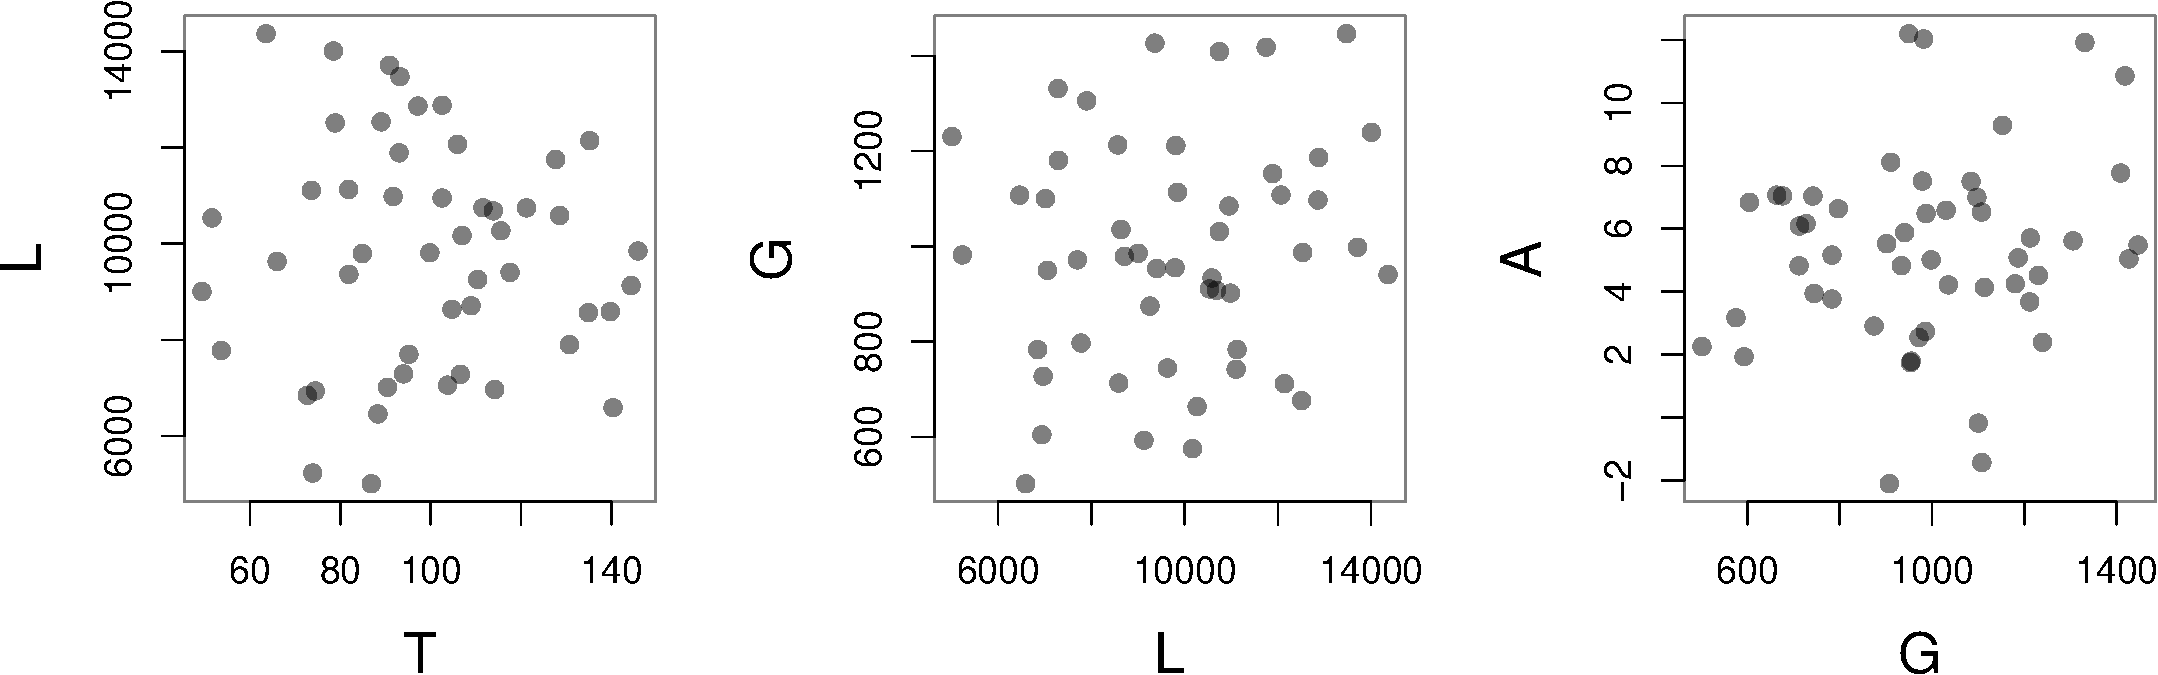
\includegraphics{main_files/figure-latex/R_block_random-1.pdf}

Plotting three of the possible combinations, we can see that the
features are essentially uncorrelated with each other and each sample is
a random distances from any other. Any inference we make from
transformations of this data must be relatable to this `ground truth'. I
now run through each of the transformations in turn, and illustrate the
difference between the actual data, and the transformed data.

\subsection{Euclidian Distance of TSS scaling transformation}

The TSS scaling transformation is simply a conversion of each sample
from a count to a proportion.

\begin{Shaded}
\begin{Highlighting}[]
\NormalTok{ran.dat.prop <-}\StringTok{ }\KeywordTok{t}\NormalTok{(}\KeywordTok{apply}\NormalTok{(ran.dat, }\DecValTok{1}\NormalTok{,}
    \NormalTok{function(x) x/}\KeywordTok{sum}\NormalTok{(x)))}

\NormalTok{dist.ran.dat.prop <-}\StringTok{ }\KeywordTok{as.matrix}\NormalTok{(}\KeywordTok{dist}\NormalTok{(}
    \NormalTok{ran.dat.prop, }\DataTypeTok{method=}\StringTok{"euclidian"}\NormalTok{))}

\KeywordTok{par}\NormalTok{(}\DataTypeTok{mfrow=}\KeywordTok{c}\NormalTok{(}\DecValTok{2}\NormalTok{,}\DecValTok{2}\NormalTok{), }\DataTypeTok{pch=}\DecValTok{19}\NormalTok{, }\DataTypeTok{col=}\KeywordTok{rgb}\NormalTok{(}\DecValTok{0}\NormalTok{,}\DecValTok{0}\NormalTok{,}\DecValTok{0}\NormalTok{,}\FloatTok{0.5}\NormalTok{),}
    \DataTypeTok{cex=}\FloatTok{1.5}\NormalTok{, }\DataTypeTok{cex.lab=}\FloatTok{1.5}\NormalTok{)}

\KeywordTok{plot}\NormalTok{(ran.dat.prop[,}\StringTok{"T"}\NormalTok{],ran.dat.prop[,}\StringTok{"L"}\NormalTok{],}
    \DataTypeTok{xlab=}\StringTok{"T.p"}\NormalTok{, }\DataTypeTok{ylab=}\StringTok{"L.p"}\NormalTok{)}
\KeywordTok{plot}\NormalTok{(ran.dat.prop[,}\StringTok{"L"}\NormalTok{],ran.dat.prop[,}\StringTok{"G"}\NormalTok{],}
    \DataTypeTok{xlab=}\StringTok{"L.p"}\NormalTok{, }\DataTypeTok{ylab=}\StringTok{"G.p"}\NormalTok{)}
\KeywordTok{plot}\NormalTok{(ran.dat.prop[,}\StringTok{"G"}\NormalTok{],ran.dat.prop[,}\StringTok{"A"}\NormalTok{],}
    \DataTypeTok{xlab=}\StringTok{"G.p"}\NormalTok{, }\DataTypeTok{ylab=}\StringTok{"A.p"}\NormalTok{)}
\KeywordTok{plot}\NormalTok{(dist.ran.dat[}\DecValTok{1}\NormalTok{,], dist.ran.dat.prop[}\DecValTok{1}\NormalTok{,],}
    \DataTypeTok{xlab=}\StringTok{"S1 vs all"}\NormalTok{, }\DataTypeTok{ylab=}\StringTok{"S1.p vs all.p"}\NormalTok{,}
    \DataTypeTok{main=}\StringTok{"Distance"}\NormalTok{)}
\end{Highlighting}
\end{Shaded}

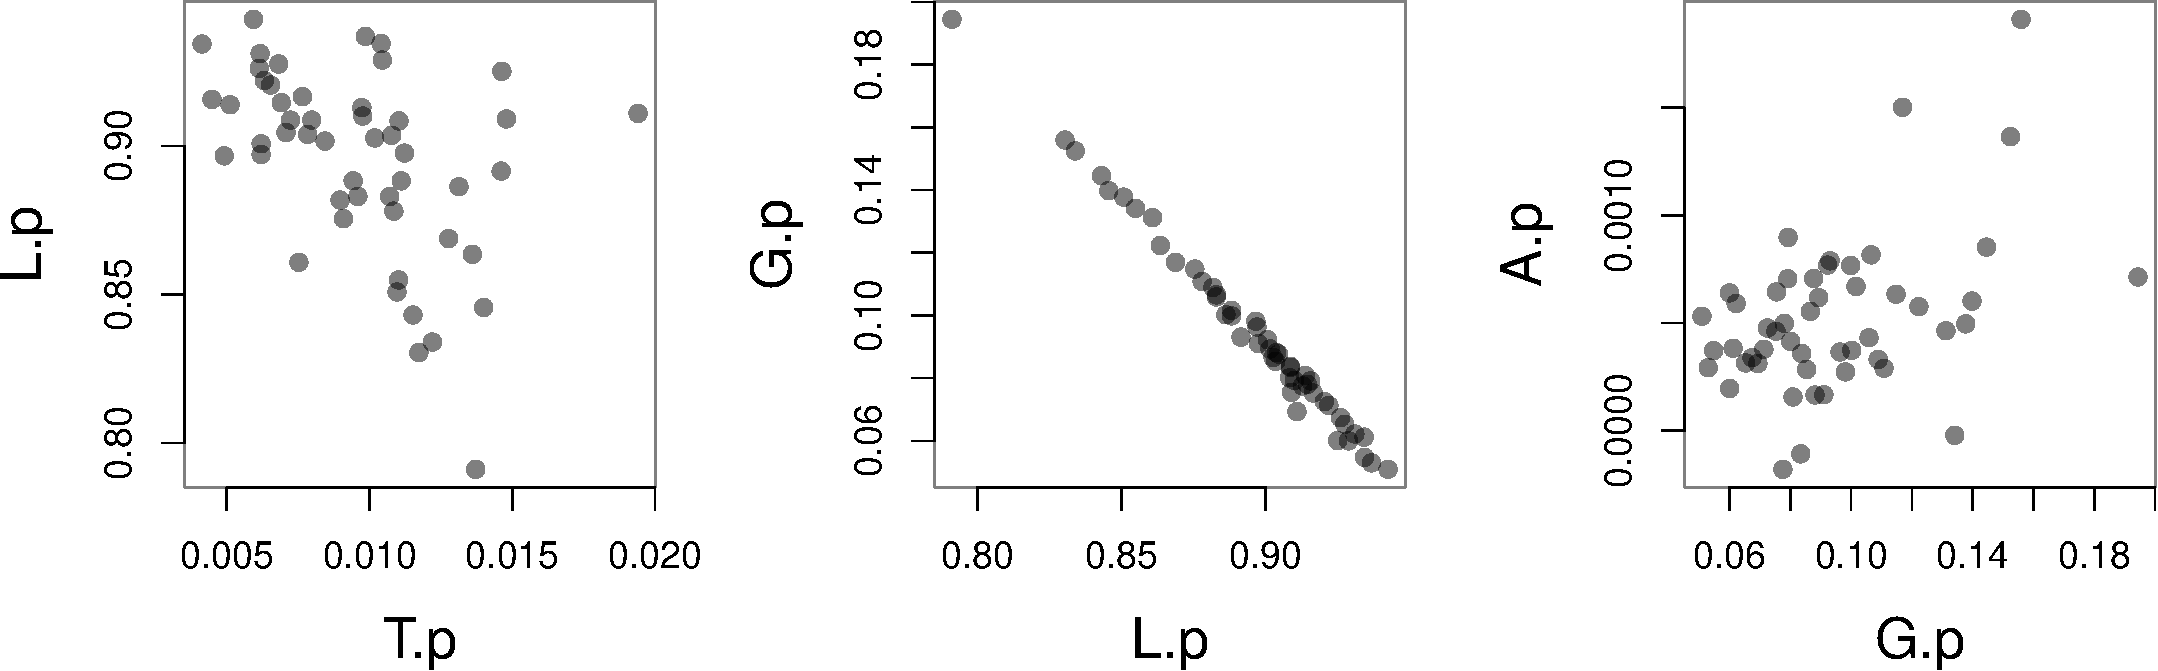
\includegraphics{main_files/figure-latex/R_block_random_prop-1.pdf}

By comparing the TSS transformed data to the non-transformed data, we
can see that the structure of the data itself has changed dramatically.
The two most abundant features, G and L, which are uncorrelated in the
actual data are now almost perfectly negatively correlated when the same
data are converted to proportions. This is because the data are now not
real numbers, but are instead proportions and are constrained by the
arbitrary sum of 1: \emph{the data are now compositional data}.

\subsection{Euclidian Distance of DM transformation}

The DM scaling transformation is a change in the scale of the sample
vector \(\vect{j}\), where each sample is scaled by a different amount.
This has the desirable property that it \emph{can} restore the a
conversion of each sample from a count to a proportion.

\begin{Shaded}
\begin{Highlighting}[]
\NormalTok{ran.dat.DM <-}\StringTok{ }\KeywordTok{t}\NormalTok{(}\KeywordTok{des.norm}\NormalTok{(}\KeywordTok{t}\NormalTok{(ran.dat.prop)))}
\NormalTok{dist.ran.dat.DM <-}\StringTok{ }\KeywordTok{as.matrix}\NormalTok{(}\KeywordTok{dist}\NormalTok{(}
    \NormalTok{ran.dat.DM, }\DataTypeTok{method=}\StringTok{"euclidian"}\NormalTok{))}

\KeywordTok{par}\NormalTok{(}\DataTypeTok{mfrow=}\KeywordTok{c}\NormalTok{(}\DecValTok{2}\NormalTok{,}\DecValTok{2}\NormalTok{), }\DataTypeTok{pch=}\DecValTok{19}\NormalTok{, }\DataTypeTok{col=}\KeywordTok{rgb}\NormalTok{(}\DecValTok{0}\NormalTok{,}\DecValTok{0}\NormalTok{,}\DecValTok{0}\NormalTok{,}\FloatTok{0.5}\NormalTok{),}
    \DataTypeTok{cex=}\FloatTok{1.5}\NormalTok{, }\DataTypeTok{cex.lab=}\FloatTok{1.5}\NormalTok{)}

\KeywordTok{plot}\NormalTok{(ran.dat.DM[,}\StringTok{"T"}\NormalTok{],ran.dat.DM[,}\StringTok{"L"}\NormalTok{],}
    \DataTypeTok{xlab=}\StringTok{"T.dm"}\NormalTok{, }\DataTypeTok{ylab=}\StringTok{"L.dm"}\NormalTok{)}
\KeywordTok{plot}\NormalTok{(ran.dat.DM[,}\StringTok{"L"}\NormalTok{],ran.dat.DM[,}\StringTok{"G"}\NormalTok{],}
    \DataTypeTok{xlab=}\StringTok{"L.dm"}\NormalTok{, }\DataTypeTok{ylab=}\StringTok{"G.dm"}\NormalTok{)}
\KeywordTok{plot}\NormalTok{(ran.dat.DM[,}\StringTok{"G"}\NormalTok{],ran.dat.DM[,}\StringTok{"A"}\NormalTok{],}
    \DataTypeTok{xlab=}\StringTok{"G.dm"}\NormalTok{, }\DataTypeTok{ylab=}\StringTok{"A.dm"}\NormalTok{)}
\KeywordTok{plot}\NormalTok{(dist.ran.dat[}\DecValTok{1}\NormalTok{,], dist.ran.dat.DM[}\DecValTok{1}\NormalTok{,],}
    \DataTypeTok{xlab=}\StringTok{"S1 vs all"}\NormalTok{, }\DataTypeTok{ylab=}\StringTok{"S1.dm vs all.dm"}\NormalTok{,}
    \DataTypeTok{main=}\StringTok{"Distance"}\NormalTok{)}
\end{Highlighting}
\end{Shaded}

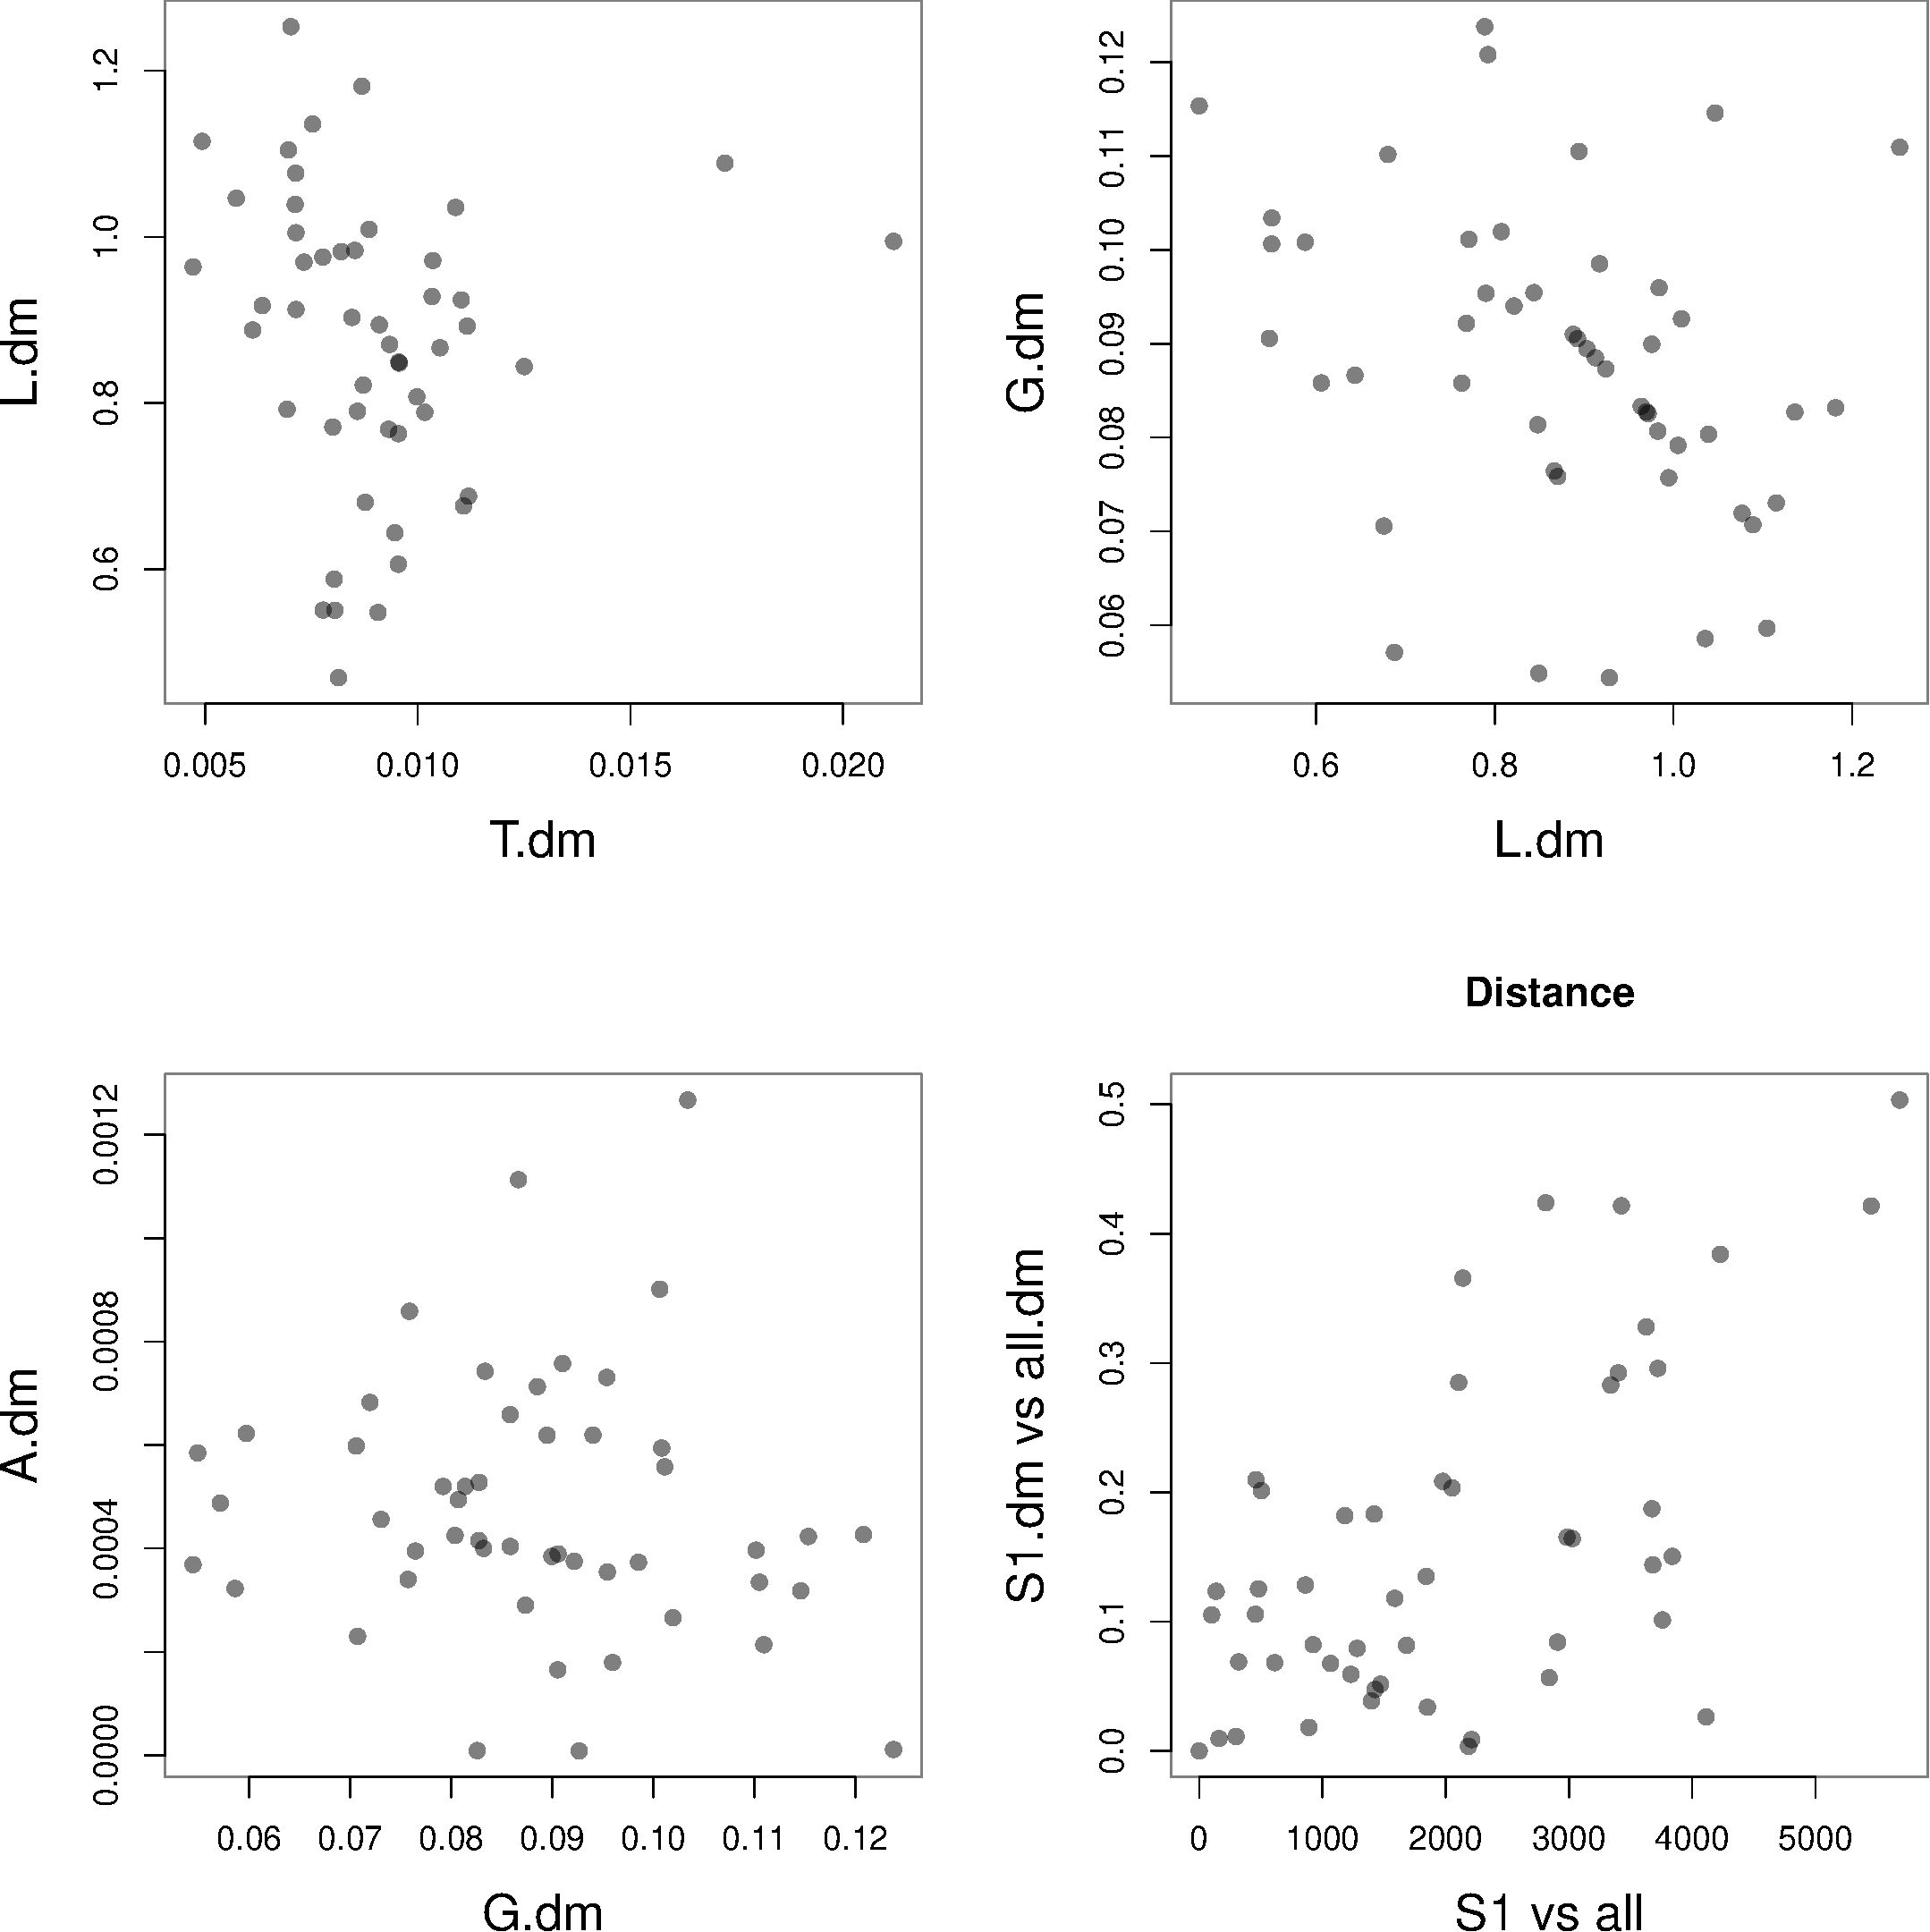
\includegraphics{main_files/figure-latex/R_block_random_DM-1.pdf}

\texttt{plot\_ly(x=ran.dat[,"L"], y=ran.dat[,"T"], z=ran.dat[,"G"])}

\texttt{plot\_ly(x=ran.dat.prop[,"L"], y=ran.dat.prop[,"T"], z=ran.dat.prop[,"G"])}

\texttt{plot\_ly(x=ran.dat.DM[,"L"], y=ran.dat.DM[,"T"], z=ran.dat.DM[,"G"])}

\subsection{Bray-Curtis Dissimilarity}\subsection{Jensen-Shannon Divergence}\subsection{Aitchison Distance}

\clearpage

\section*{References}\label{references}
\addcontentsline{toc}{section}{References}

\hyperdef{}{ref-Ait1983}{\label{ref-Ait1983}}
Aitchison, J. (1983). Principal component analysis of compositional
data. \emph{Biometrika} 70, 57--65.

\hyperdef{}{ref-Aitchison:1986}{\label{ref-Aitchison:1986}}
Aitchison, J. (1986). \emph{The statistical analysis of compositional
data}. London, England: Chapman \& Hall.

\hyperdef{}{ref-barcelo:2001}{\label{ref-barcelo:2001}}
Barceló-Vidal, C., Martín-Fernández, J. A., and Pawlowsky-Glahn, V.
(2001). ``Mathematical foundations of compositional data analysis,'' in
\emph{Proceedings of IAMG}, 1--20.

\hyperdef{}{ref-fernandes:2013}{\label{ref-fernandes:2013}}
Fernandes, A. D., Macklaim, J. M., Linn, T. G., Reid, G., and Gloor, G.
B. (2013). ANOVA-like differential expression (aLDEx) analysis for mixed
population rNA-seq. \emph{PLoS One} 8, e67019.
\href{http://doi.org/10.1371/journal.pone.0067019}{doi:10.1371/journal.pone.0067019}.

\hyperdef{}{ref-Li:2010aa}{\label{ref-Li:2010aa}}
Li, B., Ruotti, V., Stewart, R. M., Thomson, J. A., and Dewey, C. N.
(2010). RNA-seq gene expression estimation with read mapping
uncertainty. \emph{Bioinformatics} 26, 493--500.
\href{http://doi.org/10.1093/bioinformatics/btp692}{doi:10.1093/bioinformatics/btp692}.

\hyperdef{}{ref-Loven:2012aa}{\label{ref-Loven:2012aa}}
Lovén, J., Orlando, D. A., Sigova, A. A., Lin, C. Y., Rahl, P. B.,
Burge, C. B., et al. (2012). Revisiting global gene expression analysis.
\emph{Cell} 151, 476--82.
\href{http://doi.org/10.1016/j.cell.2012.10.012}{doi:10.1016/j.cell.2012.10.012}.

\hyperdef{}{ref-unifrac:2005}{\label{ref-unifrac:2005}}
Lozupone, C., and Knight, R. (2005). UniFrac: A new phylogenetic method
for comparing microbial communities. \emph{Applied and environmental
microbiology} 71, 8228--8235.

\hyperdef{}{ref-Lozupone:2011aa}{\label{ref-Lozupone:2011aa}}
Lozupone, C., Lladser, M. E., Knights, D., Stombaugh, J., and Knight, R.
(2011). UniFrac: An effective distance metric for microbial community
comparison. \emph{ISME J} 5, 169--72.
\href{http://doi.org/10.1038/ismej.2010.133}{doi:10.1038/ismej.2010.133}.

\hyperdef{}{ref-McMurdie:2014a}{\label{ref-McMurdie:2014a}}
McMurdie, P. J., and Holmes, S. (2014). Waste not, want not: Why
rarefying microbiome data is inadmissible. \emph{PLoS Comput Biol} 10,
e1003531.
\href{http://doi.org/10.1371/journal.pcbi.1003531}{doi:10.1371/journal.pcbi.1003531}.

\hyperdef{}{ref-Mortazavi:2008}{\label{ref-Mortazavi:2008}}
Mortazavi, A., Williams, B. A., McCue, K., Schaeffer, L., and Wold, B.
(2008). Mapping and quantifying mammalian transcriptomes by RNA-seq.
\emph{Nat Methods} 5, 621--8.
\href{http://doi.org/10.1038/nmeth.1226}{doi:10.1038/nmeth.1226}.

\hyperdef{}{ref-Pachter:2011}{\label{ref-Pachter:2011}}
Pachter, L. (2011). Models for transcript quantiffication from RNA-seq.
\emph{ArXiv} 1104.3889.

\hyperdef{}{ref-pawlowsky2015modeling}{\label{ref-pawlowsky2015modeling}}
Pawlowsky-Glahn, V., Egozcue, J. J., and Tolosana-Delgado, R. (2015).
\emph{Modeling and analysis of compositional data}. John Wiley \& Sons.

\hyperdef{}{ref-Robinson:2010a}{\label{ref-Robinson:2010a}}
Robinson, M. D., and Oshlack, A. (2010). A scaling normalization method
for differential expression analysis of RNA-seq data. \emph{Genome Biol}
11, R25.1--R25.9.
\href{http://doi.org/10.1186/gb-2010-11-3-r25}{doi:10.1186/gb-2010-11-3-r25}.

\hyperdef{}{ref-Silverman:2017aa}{\label{ref-Silverman:2017aa}}
Silverman, J. D., Washburne, A. D., Mukherjee, S., and David, L. A.
(2017). A phylogenetic transform enhances analysis of compositional
microbiota data. \emph{Elife} 6, 21887.
\href{http://doi.org/10.7554/eLife.21887}{doi:10.7554/eLife.21887}.

\hyperdef{}{ref-Vandesompele:2002aa}{\label{ref-Vandesompele:2002aa}}
Vandesompele, J., De Preter, K., Pattyn, F., Poppe, B., Van Roy, N., De
Paepe, A., et al. (2002). Accurate normalization of real-time
quantitative rT-pCR data by geometric averaging of multiple internal
control genes. \emph{Genome Biol} 3, RESEARCH0034.

\hyperdef{}{ref-Wong:2016aa}{\label{ref-Wong:2016aa}}
Wong, R. G., Wu, J. R., and Gloor, G. B. (2016). Expanding the UniFrac
toolbox. \emph{PLoS One} 11, e0161196.
\href{http://doi.org/10.1371/journal.pone.0161196}{doi:10.1371/journal.pone.0161196}.

\end{document}
